\scanpage{71}
% archive sheet number: 70
\[
\boxed{F(X,Y,Z)=(-X+Y+Z)^2-4(\alpha+2)YZ+\underbrace{\frac{2-\alpha}{4(\alpha+2)}}_{\deleted{\unsure{\beta''|\rho''}}\ \lambda>0}}
\]
% The lower border of the formula box crosses this parenthesis; no independent cancellation is resolved.
(Origine reportée à $o$)
\[
\begin{aligned}
-2<\alpha<2\\
0<4(\alpha+2)<16
\end{aligned}
\]
\[
4YZ=(Y+Z)^2-(Y-Z)^2
\qquad
\left\{\begin{aligned}
\deleted{\unsure{\rho}}-X+Y+Z&=\deleted{\unsure{W}}U\sqrt{\lambda}\\
\sqrt{\alpha+2}(Y+Z)&=\deleted{V}W\sqrt{\lambda}\\
\sqrt{\alpha+2}(Y-Z)&=\deleted{W}V\sqrt{\lambda}
\end{aligned}\right.
\]
\[
\unsure{G|E}(U,V,W)=U^2\deleted{\unsure{-}}+\deleted{\unsure{\frac{(\alpha+2)}{\rho}}}(\deleted{\unsure{W}}V^2-\deleted{\unsure{V}}W^2)+\deleted{\underbrace{\frac{2-\alpha}{4(\alpha+\unsure{2|\beta})}}_{\lambda}}1
\]
\[
\deleted{\rho,\unsure{\sigma}\ge0}
\qquad\begin{aligned}
U^2+V^2-W^2+\deleted{\lambda}1&=0\\
u^2&=v^2+w^2+\unsure{\lambda}
\end{aligned}
\]
\[
\deleted{W^2-\rho UV+\sigma=0}\qquad\deleted{\rho\unsure{UW|UV}=W^2+\sigma}
\]
\[
\deleted{W^2-\rho U\deleted{W}V}\qquad
\deleted{\unsure{\rho}\quad W^2-\rho YZ+\sigma=0}
\]
\[
\deleted{\rho YZ=W^2+\sigma}
\qquad W^2=U^2+V^2+1
\]
\figure{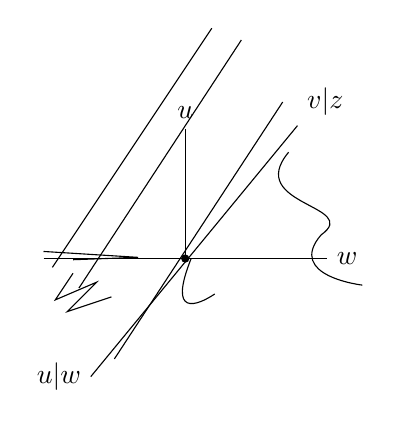
\begin{tikzpicture}[scale=.75]
\draw (-2.4,0)--(2.4,0);
\draw (0,0)--(0,2.2);
\draw (-1.6,-2)--(1.9,2.25);
\fill (0,0) circle (2pt);
\node[above] at (0,2.2) {$\unsure{u}$};
\node[above right] at (1.9,2.25) {$\unsure{v|z}$};
\node[right] at (2.4,0) {$\deleted{\unsure{w}}$};
\node[left] at (-1.6,-2) {$\deleted{\unsure{u|w}}$};
\draw (-2.25,-.15)--(.45,3.9);
\draw (-1.8,-.5)--(.95,3.7);
\draw (-1.2,-1.7)--(1.65,2.65);
\draw (-2.4,.12)--(-.8,.02)--(-1.9,-.02);
\draw (1.75,1.8) .. controls (1.0,.9) and (3,.9) .. (2.3,.4) .. controls (1.7,-.3) and (3,-.45) .. (3,-.45);
\draw (.1,0) .. controls (-.3,-1) and (.2,-.8) .. (.5,-.6);
\draw (-1.9,-.25)--(-2.2,-.7)--(-1.5,-.4)--(-2,-.9)--(-1.25,-.65);
\end{tikzpicture}}
\figure{\begin{tikzpicture}[scale=.85]
\draw (0,0)--(0,1.8) node[above] {$w$};
\draw (0,0)--(1.8,-.25) node[right] {$V$};
\draw (0,0)--(-1.25,-1.65) node[below left] {$\unsure{u|U}$};
\end{tikzpicture}}
